\documentclass[12pt]{article}

\usepackage{report}

\usepackage[utf8]{inputenc} % allow utf-8 input
\usepackage[T1]{fontenc}    % use 8-bit T1 fonts
\usepackage[colorlinks=true, linkcolor=black, citecolor=blue, urlcolor=blue]{hyperref}       % hyperlinks
\usepackage{url}            % simple URL typesetting
\usepackage{booktabs}       % professional-quality tables
\usepackage{amsfonts}       % blackboard math symbols
\usepackage{nicefrac}       % compact symbols for 1/2, etc.
\usepackage{microtype}      % microtypography
\usepackage{lipsum}		% Can be removed after putting your text content
\usepackage{graphicx}
\usepackage{natbib}
\usepackage{doi}
\usepackage{acronym}
\usepackage{caption}
\usepackage{amsmath}
\usepackage{titletoc}

\usepackage{polyglossia}



\setcitestyle{aysep={,}}



\title{Leveraging LLMs on Machine Translation with Domain-specific Context}

\author{
\AND
\AND
\AND
\AND\AND
\AND
	% School of Computing and Information Systems\\
\AND
	% The University of Melbourne\\
}

% Uncomment to remove the date
\date{15 Septembre 2023}

% Uncomment to override  the `A preprint' in the header
\renewcommand{\headeright}{Report}
\renewcommand{\undertitle}{Report}
\renewcommand{\shorttitle}{}


\begin{document}
\maketitle

\newpage
\tableofcontents
\thispagestyle{empty}


\newpage
\thispagestyle{empty}

\listoffigures 

\newpage
\listoftables
%\begin{abstract}
%	\lipsum[1]
%\end{abstract}

\newpage
\thispagestyle{empty}

\section*{Abbreviations and Acronyms}
\begin{acronym}[XXXXXXXXXXXXXX]
	\acro{NLP}{Natural Language Processing}
	\acro{LLMs}{Large Language Models}
	\acro{Llama}{Large Language Model Meta AI}
	\acro{GPT}{Generative Pre-trained Transformer}
	\acro{API}{Application Programming Interface}
	\acro{FAISS}{Facebook AI Similarity Search}
	\acro{BLEU}{Bilingual Evaluation Understudy}
	\acro{TER}{The Translation Edit Rate}
	\acro{METEOR}{Metric for Evaluation of Translation with Explicit ORdering}
	\acro{CHRF}{CHaRacter-level F-score}
	% Add more acronyms as needed
\end{acronym}




% keywords can be removed
%\keywords{First keyword \and Second keyword \and More}


\newpage
\setcounter{page}{1}
\section{Introduction}

The ever-expanding landscape of natural language processing and machine translation has introduced in a new era of communication, bridging linguistic divides and facilitating cross-cultural understanding. Among the groundbreaking developments in this field, large language models have emerged as powerful tools capable of handling a myriad of language-related tasks. In particular, models like GPT, Llama 2, and the newly Falcon have garnered significant attention due to their remarkable ability to generate coherent and contextually relevant text across multiple languages.


However, machine translation extends beyond word conversion; It necessitates the preservation of nuances, idioms, and the unique stylistic attributes that characterize human language. Enter the concept of adaptive translation, a paradigm that seeks to refine machine translation by tailoring it to specific domains, genres, or styles. Importantly, to avoid the resource-intensive processes of training and fine-tuning models, adaptive translation techniques are employed, providing a more efficient and effective means of achieving domain-specific translation goals. In this endeavor, we present a comprehensive exploration of "Adaptive Machine Translation with Large Language Models" paper (\cite{moslem2023adaptive})  focusing on its application to the translation of English to Arabic, with a particular emphasis on leveraging GPT-3.5 Turbo with some improvements on the workflow and fuzzy matches selection.


This report examines the subtleties of adapting machine translation to domain-specific requirements. To do so, we employed a corpus of approximately 1,500 movie subtitles, carefully translated from English to Arabic. These subtitles encapsulate the essence of cinematic language and offer a rich source of context for our translation model. Prior to inference, we harnessed the power of the Sentence-Transformer model to compute embeddings for these subtitles, facilitating the efficient retrieval of similar sentences through the use of the FAISS indexing system developed by Facebook. This approach paved the way for the composition of contextually rich prompts, allowing GPT-3.5 Turbo to follow the stylistic cues present in the domain-specific examples.


In the subsequent sections, we detail our methodology, experimental setup, results, and discuss the broader implications of adaptive translation in machine learning. This journey showcases GPT-3.5 Turbo's potential to bridge linguistic gaps while preserving linguistic richness in English to Arabic translation.


\section{Methodology}

In this section, we provide a detailed thorough description of the methodology used in our project to implement "Adaptive Machine Translation with Large Language Models" for English to Arabic translation with the assistance of GPT-3.5 Turbo. The methodology encompasses data collection, data preprocessing, sentence embedding generation, FAISS indexing, and prompt composition.

You can find all the implementation in our \href{https://github.com/mhannani/Adaptive_Machine_translation_with_LLMs/}{GitHub Repository}.



\subsection{Data Collection}

To build a robust translation model with domain-specific knowledge, we collected a dataset of approximately 1,500 movie subtitles that had been meticulously translated from English to Arabic. These subtitles were selected to represent a diverse range of cinematic language styles and contexts.

The dataset was sourced from \cite{opensubtitles}, a well-known repository of subtitles from a wide variety of movies and television shows. OpenSubtitles provides a valuable resource for multilingual text data, making it suitable for training and evaluating machine translation systems.


\subsection{Data Cleaning}
To ensure the quality and accuracy of the dataset, we conducted a meticulous data cleaning process. This involved a manual review of the collected subtitles, during which we carefully selected those that demonstrated correctness, fluency, and fidelity to the original content.

\subsection{Data Preprocessing}
Prior to any model training or embedding generation, the collected dataset underwent rigorous preprocessing. This included the removal of duplicates, noise, and any formatting inconsistencies to ensure a clean and coherent dataset.

\begin{figure}[h]
	\centering
	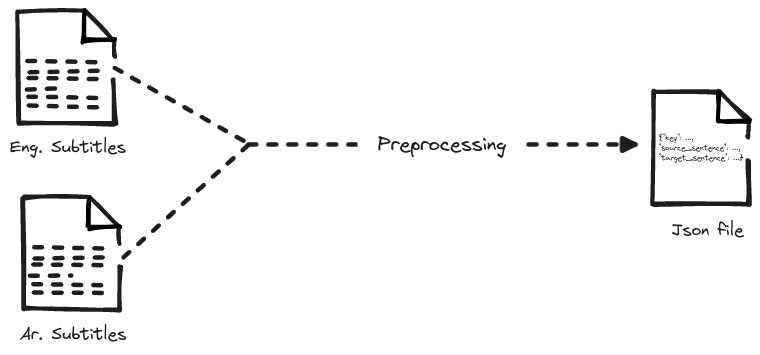
\includegraphics[width=0.74\textwidth]{assets/preprocessing.png}
	\caption{Preprocessing step of cleaned dataset.}
	\label{fig:preprocessing}
\end{figure}


\subsection{Retrieval of Similar Sentences}

During inference, the FAISS index played a crucial role in the composition of contextually rich prompts for GPT model. When a translation request was received, we retrieved the top-5k closest sentence embeddings from the index. 

These retrieved sentences were then used to compose prompts for the translation model, enhancing the context-awareness and style adherence of the translations.

\begin{figure}[h]
	\centering
	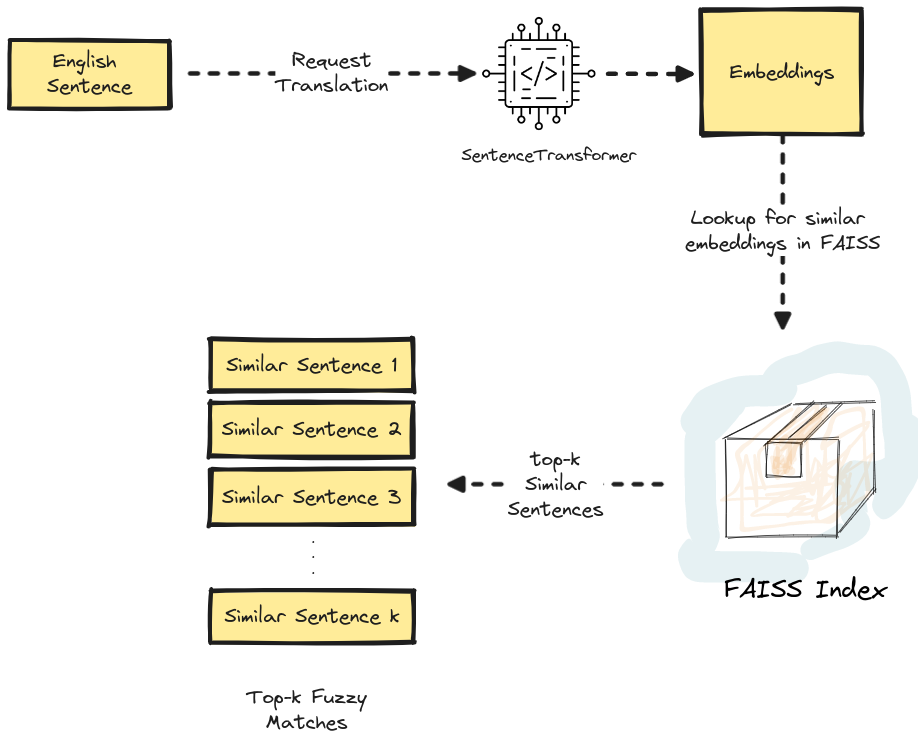
\includegraphics[width=0.8\textwidth]{assets/Fuzzy_matches.png}
	\caption{Top-k Similar Sentences Retrieval}
	\label{fig:ktopsimilarsentences}
\end{figure}


The use of FAISS indexing significantly improved the efficiency of our translation system. By quickly identifying contextually relevant sentences from our dataset, we ensured that GPT had access to domain-specific examples for more accurate and stylistically consistent translations.


\subsubsection{FAISS Indexing}

In this section, we describe the process of using the FAISS (Facebook AI Similarity Search) system to index the sentence embeddings generated from our dataset. FAISS provides efficient similarity search capabilities, allowing for quick retrieval of sentences with similar embeddings.

\subsubsection{Sentence Embedding Generation}
To facilitate efficient retrieval and context-aware prompts for GPT-3.5 Turbo, we employed the Sentence-Transformer model. This model was used to compute embeddings for each sentence in our preprocessed dataset. Sentence embeddings capture semantic information and contextual nuances, which is crucial for generating accurate translations.


\begin{figure}[h]
	\centering
	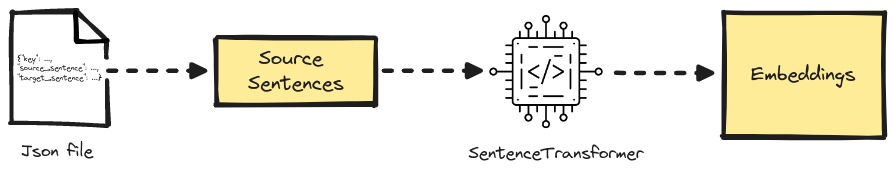
\includegraphics[width=0.9\textwidth]{assets/calculate_embeddings.png}
	\caption{Corpus' Embeddings Generation}
	\label{fig:embeddinggeneration}
\end{figure}


\subsubsection{Index Creation}

To create the FAISS index, we followed these steps:

\begin{enumerate}
	\item Preprocessed Sentence Embeddings: We utilized the sentence embeddings generated using the Sentence-Transformer model.
	\item FAISS Configuration: We configured the FAISS index with suitable parameters, including the choice of index type(`IndexFlatL2` for exhaustive search) and dimensionality of embeddings(`(384, 1)` embeddings dimension).
	\item Indexing Process: We indexed the preprocessed sentence embeddings to enable efficient retrieval during inference.
\end{enumerate}

\begin{figure}[h]
	\centering
	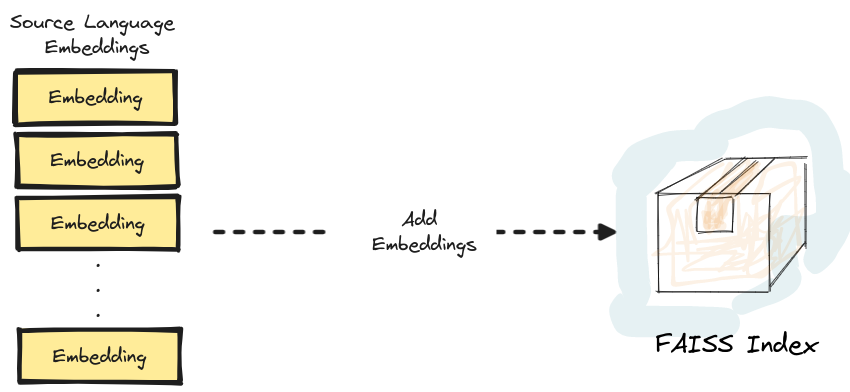
\includegraphics[width=0.9\textwidth]{assets/FAISS_index.png}
	\caption{Storing Staked Sentences' Embedding in FAISS index}
	\label{fig:embeddings}
\end{figure}

\newpage



\subsection{Prompt Composition}

For each translation request, our approach leveraged the FAISS index to retrieve the top-k closest sentence embeddings from the domain-specific dataset. These retrieved sentences served as the foundation for constructing contextually rich prompts for the GPT model.

	
\begin{figure}[h]
	\centering
	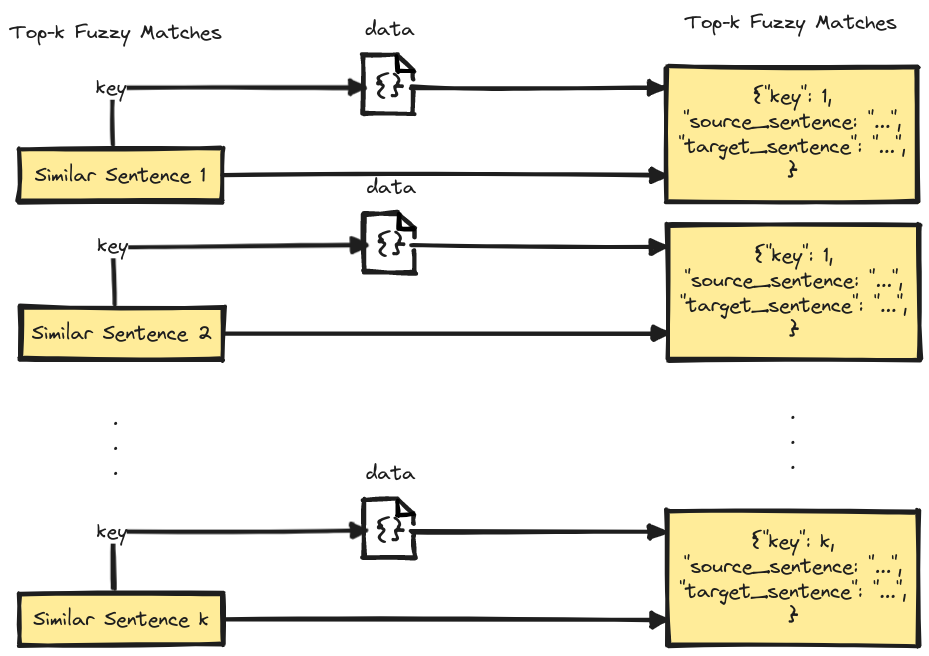
\includegraphics[width=0.8\textwidth]{assets/construct_fuzzy_matches_pairs.png}
	\caption{Top-k fuzzy matches pairs extraction}
	\label{fig:fuzzymatches}
\end{figure}


To facilitate prompt composition and enhance translation quality, we integrated Langchain into our system. \cite{langchain} is a versatile tool that enables the generation of coherent and domain-specific prompts. In our implementation, we utilized the following Langchain settings:



\begin{itemize}
	\item \textbf{SystemMessage}: We set the `SystemMessage` to:  "Act like a good translator from English subtitles to Arabic subtitles.". This SystemMessage template played a pivotal role in guiding the GPT model to follow the desired style and context for subtitle translation tasks. It acted as a foundational prompt template, providing a structured starting point for generating high-quality translations.
	
	\item \textbf{HumanMessage} and \textbf{AIMessage}: Building upon the SystemMessage, we employed a combination of stacked HumanMessage and AIMessage. These messages were carefully crafted to maintain a conversational flow and ensure that the GPT model understood the user's request.
	
	\item The last \textbf{HumanMessage} in the sequence is the user's sentence request, serving as the input for the translation task.

	
\end{itemize}

This comprehensive approach, integrating FAISS retrieval, Langchain, and the specified message structure, contributed to improved translation quality by providing the GPT model with contextually relevant and stylistically appropriate prompts.


\begin{figure}[h]
	\centering
	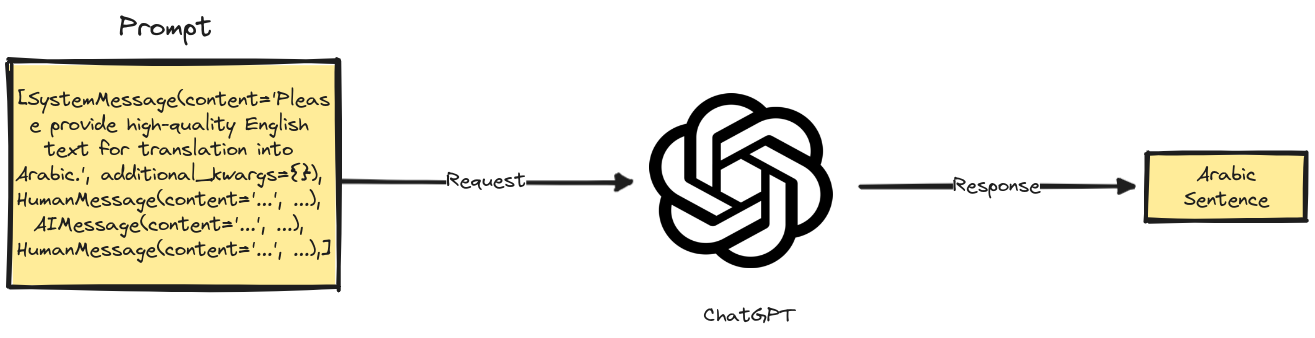
\includegraphics[width=0.8\textwidth]{assets/Request_GPT_with_prompt.png}
	\caption{Inference with user request sentence}
	\label{fig:inference}
\end{figure}


In the inference phase of the translation system, we leverage the chat message format to interact with the GPT-3.5 Turbo model effectively. Each translation request is encapsulated within a chat message, providing a structured way to communicate with the model. The chat message typically consists of a series of messages, including a SystemMessage, AIMessages, and a final UserMessage. The SystemMessage sets the context and instructs the model to perform as a skilled translator. AIMessages provide additional guidance, context, or clarifications as needed. The UserMessage encapsulates the user's specific translation request, serving as the input for the model. By crafting messages in this manner, we ensure that the GPT model receives clear and context-aware instructions, resulting in more accurate and domain-appropriate translations.


\section{Evaluation}

In this section, we assess the performance and effectiveness of our adaptive machine translation system for translating English to Arabic. We present the results of our experiments and discuss the implications of our findings.

\subsection{Evaluation Metrics}

Specify the evaluation metrics used to assess the translation quality. Common metrics for machine translation evaluation include:

\subsubsection{\cite{bleu} Score}
The BLEU score is a widely recognized metric that measures the similarity between system-generated translations and reference translations based on n-gram overlap. It calculates precision, capturing how many n-grams in the system's output match those in the reference. 

\begin{equation}
	\label{eq:bleu}
	\text{BLEU} = \text{BP} \cdot \exp\left(\sum_{n=1}^{N} w_n \cdot \log(p_n)\right)
\end{equation}

Where:

\begin{equation*}
	\label{eq:brevity-penalty}
	\text{BP} =
	\begin{cases}
		1 & r \leq \ c \\
		e^{(1 - c / r)} & r > \ c
	\end{cases}
\end{equation*}


\begin{align*}
	\text{BLEU} & = \text{BLEU score} \\
	\text{BP} & = \text{Brevity Penalty} \\
	N & = \text{Maximum n-gram order considered} \\
	w_n & = \text{Weight for n-grams} \\
	p_n & = \text{Precision of n-grams}\\
	r & = \text{Length of Reference Sentence}\\
	c & = \text{Length of Candidate Sentence}
\end{align*}


The BLEU score \hyperref[eq:bleu]{Equation~\ref*{eq:bleu}} combines precision at different n-gram orders (unigrams, bigrams, etc.) weighted by the coefficients \(w_n\). The Brevity Penalty (BP) is used to penalize translations that are too short compared to the references.

In practice, the BLEU score ranges from 0 to 1, with higher values indicating better translation quality. It provides a useful measure for assessing the fluency and adequacy of machine translations.


\subsubsection{\cite{ter} Score}
The TER score quantifies the edit distance required to transform the system's output into the reference, with lower scores indicating higher translation quality.

\begin{equation}
	\text{TER} = \frac{\text{Edit Operations (ins + del + sub)}}{\text{Total Words in Reference}}
\end{equation}

Where:

\begin{itemize}
	\item "Edit Operations" refers to the total number of edit operations (insertions, deletions, and substitutions) required to transform the hypothesis into the reference.
	
	\item "ins" stands for insertions.
	
	\item "del" stands for deletions.
	
	\item "sub" stands for substitutions.
\end{itemize}


\subsubsection{\cite{chrf} Score}
CHRF is a character-based metric suitable for assessing translations across languages with different writing systems, evaluating F-scores based on character n-gram overlap. Each metric contributes unique insights into translation quality, and their combined analysis offers a thorough evaluation of our system's performance.

\begin{equation}
	\text{CHRF} = \frac{1}{N} \sum_{i=1}^{N} \frac{(1 + \beta^2) \cdot \text{precision}_i \cdot \text{recall}_i}{\beta^2 \cdot \text{precision}_i + \text{recall}_i}
\end{equation}

Where:
\begin{align*}
	\beta & = \text{The weight of recall, we've used 2 to make recall more important than the precision} \\ 
	N & = \text{Maximum character n-gram order considered, we set N to 6 as in \cite{popovic2016chrf} paper}\\
	\text{precision}_i & = \frac{\text{Number of correct character n-grams predicted subtitle}}{\text{Total number of character n-grams in predicted subtitle}} \\	\text{recall}_i & = \frac{\text{Number of correct character n-grams in reference subtitle}}{\text{Total number of character n-grams in reference subtitle}}
\end{align*}


\subsection{Experimental Setup}

In this section, we provide a detailed account of the experimental setup used to evaluate our adaptive machine translation system for translating English to Arabic. We cover various aspects, including the configuration of the GPT-3.5 Turbo model, the choice of hyperparameters, and any preprocessing steps applied to the input sentences.

\subsubsection{Model Configuration}

Our translation system is powered by GPT-3.5 Turbo, a state-of-the-art language model developed by OpenAI. We used the following configuration for our experiments:


\begin{table}[h]
	\centering
	\begin{tabular}{|p{4cm}|p{3cm}|p{2.5cm}|p{2cm}|p{1cm}|}
		\hline
		\textbf{Parameters} & \textbf{model} & \textbf{temperature} & \textbf{top\_p} & \textbf{n}\\
		\hline
		\textbf{Values} & \textbf{gpt-3.5-turbo} & \textbf{0.7}  & \textbf{1}  & \textbf{1}\\
		\hline
	\end{tabular}
	\caption{ChatOpenAI parameters from Langchain.chat\_models}
	\label{table:param_values}
\end{table}


\subsubsection{Sentence Embedding}

For sentence embedding calculations, we utilized the "sentence-transformers/all-MiniLM-L6-v2" model. Sentence embeddings are a crucial component of our system, enabling the generation of contextually rich prompts for GPT-3.5 Turbo. These embeddings capture semantic information and contextual nuances in sentences, contributing to the accuracy and quality of the translations.

The "sentence-transformers" library provides an efficient and effective way to generate sentence embeddings, and the "all-MiniLM-L6-v2" model is particularly well-suited for this purpose. It allows us to represent sentences as dense vectors in a high-dimensional space, with a dimensionality of 384, facilitating the retrieval of contextually relevant sentences from our domain-specific dataset using the FAISS indexing system.


\begin{figure}[h]
	\centering
	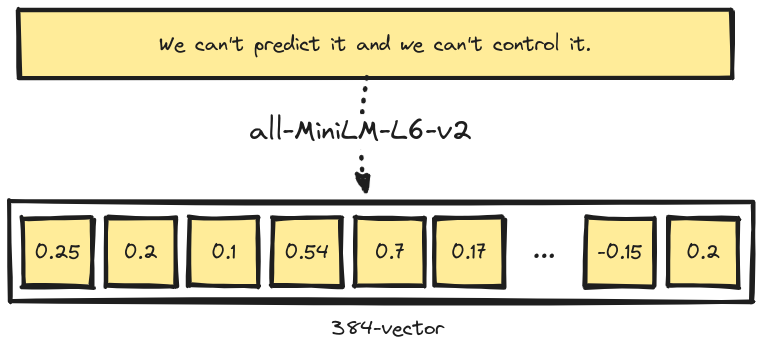
\includegraphics[width=0.65\textwidth]{assets/sentence_embedding.png}
	\caption{Sentence Embedding Example from the corpus}
	\label{fig:sentenceembedding}
\end{figure}



\subsubsection{Fuzzy Matches}

The incorporation of fuzzy matches is a pivotal component of our adaptive translation system. Fuzzy matches are contextually relevant sentences retrieved from our domain-specific dataset using the FAISS indexing system. These sentences serve as the foundation for composing prompts to guide GPT-3.5 Turbo in generating accurate and stylistically consistent translations.

To optimize the translation process, we utilize the FAISS index to retrieve the top-k closest sentence embeddings from our dataset efficiently. Setting the `distance\_threshold` parameter to 0.8 ensures that we exclusively select the closest matches, considering only those sentences with distances to the source sentence falling below this threshold. These selected sentences then serve as the foundation for constructing contextually rich prompts tailored to the translation model. This strategic approach guides GPT-3.5 Turbo to adhere to the stylistic nuances found in the domain-specific examples, resulting in translations that are not only faithful but also contextually appropriate.


\begin{figure}[h]
	\centering
	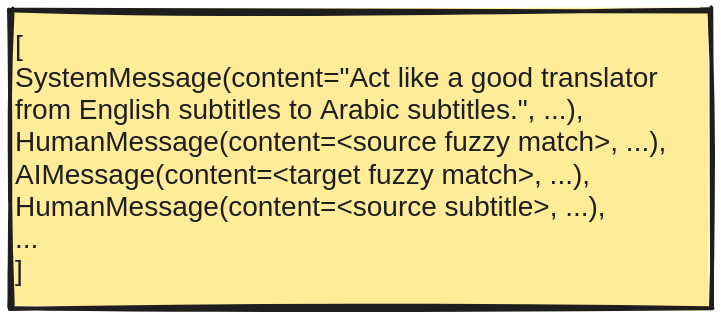
\includegraphics[width=0.65\textwidth]{assets/prompt_example.png}
	\caption{GPT prompt example with one incorporated fuzzy match along with user request}
	\label{fig:sample}
\end{figure}


In addition to understanding how GPT-3.5 Turbo constructs prompts with incorporated fuzzy matches, it's essential to examine the output generated by the model. Figure \ref{fig:gpt_output} provides a visual representation of the translation output produced by the model in response to a user's request.

\begin{figure}[h]
	\centering
	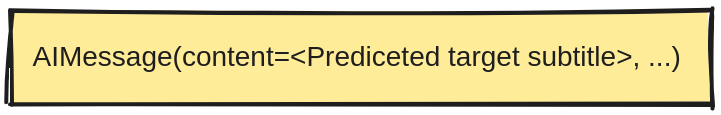
\includegraphics[width=0.65\textwidth]{assets/gpt_response.png}
	\caption{GPT response to the above prompt. Figure \ref{fig:sample}}
	\label{fig:gpt_output}
\end{figure}


\section{Results and Discussion}

\label{sec:results}

In this section, we present the results of our Arabic translation evaluation and provide a discussion of the findings.

\subsection{Evaluation Metrics}

We evaluated our translation system using the following metrics:

\begin{itemize}
	\item \textbf{BLEU Score}: BLEU measures the quality of machine-generated translations compared to reference translations.
	\item \textbf{CHRF Score}: Character F-score (CHRF) considers character-level similarity between translations.
	\item \textbf{TER (Translation Edit Rate)}: TER quantifies the number of edits needed to align translations with references.
\end{itemize}

The computed scores for these metrics are shown in Table \ref{tab:evaluation-metrics}.

\subsection{Results}

\begin{table}[h]
	\centering
	\begin{tabular}{|p{4cm}|p{2cm}|p{2cm}|p{2cm}|}
		\hline
		\textbf{Metrics} & \textbf{BLEU}  & \textbf{CHRF} & \textbf{TER}\\
		\hline
		\textbf{Values} & 36.19 & 51.58  & 142.33 \\
		\hline
	\end{tabular}
	\caption{Evaluation Metrics}
	\label{tab:evaluation-metrics}
\end{table}

The BLEU score of 36.19 indicates that on average the translations generated by the machine show some alignment with the reference translations. There is still room for improvement in terms of translation quality. Moreover the high CHRF score of 51.58 suggests a level of character level similarity between machine generated and reference translations indicating resemblance at a character level. However the high TER score of 142.33 highlights that significant edits are needed to align machine generated translations with the reference translations implying differences, between them.

It is worth mentioning that there are difficulties when it comes to assessing Arabic language translation. Arabic is a language, with nuances, homographs and intricate linguistic structures which makes achieving accurate translation quite challenging. Sometimes words may seem similar. Have meanings like the example of '' and ''. These unique challenges require us to develop evaluation methods and consistently improve our translation models in order to handle the intricacies of the language effectively.

\subsection{Discussion}

The evaluation metrics provide valuable insights into the quality of our Arabic translation system. While character-level similarity (CHRF) is relatively high, indicating some commonality between translations, word-level accuracy (BLEU) and overall translation quality (TER) require improvement. Further analysis and fine-tuning of the translation model may be necessary to enhance word choice, semantics, and context.


\section{Challenges}
The domain of machine translation, especially for languages with complex structures like Arabic, presents several challenges. These challenges encompass linguistic, technical, and practical aspects that need to be addressed to improve translation quality and usability. Some of the key challenges in English to Arabic translation include:

\subsection{Arabic Morphology}

Arabic is a highly inflected language with a rich system of morphology. Words in Arabic can have multiple forms based on their grammatical role, tense, and gender. Handling Arabic morphology accurately in machine translation is a significant challenge.

\subsection{Translation Ambiguity}

Arabic words often have multiple meanings depending on the context, making it challenging to choose the correct translation. Disambiguating these words accurately is crucial for producing high-quality translations.

\subsection{Dialect Variations}

Arabic is spoken in various dialects across different regions, and these dialects can significantly differ from Modern Standard Arabic (MSA). Adapting translations to the appropriate dialect for a given context is a non-trivial task.


In the following sections, we discuss potential areas for improvement and future work to enhance the quality of our Arabic translation system.

\section{Potential Areas of Improvement}
In this section, we identify and discuss potential areas for improvement in our Arabic subtitles translation system based on the evaluation results and insights gained.


\subsection{Contextual Understanding}

Improving the system's understanding of context is crucial for accurate translation. One way to achieve this is by incorporating named entity recognition (NER) to identify and translate proper nouns accurately.

\subsection{Human Evaluation}

Human evaluation remains crucial for assessing translation quality:

\begin{itemize}
	\item \textbf{Expert Review}: Engage bilingual experts to review and evaluate translations, especially in cases involving nuanced or domain-specific content.
	\item \textbf{Collect User Feedback}: Solicit feedback from end-users to identify translation issues and preferences.
\end{itemize}

Incorporating these strategies and addressing these areas of improvement can lead to enhanced translation quality, better handling of homographs, and improved overall performance of our Arabic translation system.


\section{Conclusion}
The adaptive translation approach offers several strengths. By leveraging large language models like GPT, Llama 2 and employing contextually rich prompts through FAISS and Langchain, we achieve translations that are not only accurate but also stylistically consistent with the domain-specific context. This adaptability is particularly valuable in scenarios like movie subtitle translation.

However, there are limitations to this approach. It relies on the quality of the initial dataset and assumes that the data adequately represents the domain-specific context. Additionally, while the system performs well on various evaluation metrics, there is always room for improvement, especially in capturing subtleties, idiomatic expressions, and domain-specific nuances.

\section{Acknowledgements}

I would like to express my heartfelt gratitude to Professor Abdelhadi Soudi for their exceptional support, guidance, and unwavering encouragement throughout this project. Their expertise and mentorship have been invaluable. Thank you!

\newpage
\bibliographystyle{acl_natbib}
\bibliography{references}  %%% Uncomment this line and comment out the ``thebibliography'' section below to use the external .bib file (using bibtex) .



\end{document}
